\documentclass[11pt,a4paper,twoside,pdf]{article}

% Paquetes (añade otros si los necesitas):

\usepackage[T1]{fontenc}
\usepackage[utf8]{inputenc}


\usepackage[pdftex,final]{graphicx}

% Style package
% Font Package (Palatino)
\usepackage{mathpazo}
% Packages for specific capabilities
\usepackage{rotating} % for text rotation in tables
\usepackage{multirow} % for multirow in tables
\usepackage{subfigure} % Place subfigures in figure environment
% Packages for specific symbols
\usepackage{amssymb}
\usepackage{amsmath}
\usepackage{amsfonts}
\usepackage{eurosym} % Euro symbol
\usepackage{bbding} % for \XSolidBrush
\usepackage{pifont} % for \ding{55} (a check mark)


\usepackage{latexsym}
\usepackage{soul}
\usepackage{array}
%\usepackage{marvosym}
\usepackage{epsfig}
\usepackage{graphics}
\usepackage{amsfonts}
\usepackage{xspace}
\usepackage{color}
\usepackage{booktabs}
\usepackage{xtab}
\usepackage[colorlinks=true,urlcolor=blue,linkcolor=blue,citecolor=blue]{hyperref}
\numberwithin{equation}{section}

\usepackage{lipsum}
\usepackage{pict2e}
\usepackage{wrapfig}
\usepackage{minted}

\linespread{1.05}

% TFG en inglés:
%\usepackage[english]{babel} 
%\addto\captionsenglish{\renewcommand{\chaptername}{}}

% TFG en español:
\usepackage[spanish,es-nodecimaldot,es-tabla,es-lcroman,es-nosectiondot,
            es-noindentfirst]{babel}
\renewcommand\spanishchaptername{}

% Formato de la página:
\usepackage{fancyhdr}
\usepackage[top=2.88cm,bottom=2.97cm,left=2.95cm,right=2.95cm]{geometry}
\setlength{\parskip}{0.1cm}

% Pon aquí tus definiciones:

\newcommand{\dis}{\displaystyle}
%\sodef\an{}{.2em}{1em plus1em}{2em plus.1em minus.1em}

\begin{document}

% Portada %%%%%%%%%%%%%%%%%%%%%%%%%%%%%%%%%%%%%%%%%%%%%%%%%%%%%%%%%%%%%%%%%%%%%%

\pagestyle{empty}


\noindent
\begin{tabular}{r}

\includegraphics[width=8.8cm]{img/escudoUGRmonocromo.png} \\[-1.8ex]
\hspace{31mm}\vspace{-8mm}
\begin{tabular}{c}
\hline\\[-1ex]\hskip-2mm
{\bf Facultad de Ciencias}\hspace{18mm}
\end{tabular}
\end{tabular}

\large
\vspace{30mm}
\hspace{25mm}
\begin{tabular}{l}
GRADO EN F\'ISICA
\end{tabular}

\vspace{45mm}
\hspace{25mm}
\begin{tabular}{l}
TRABAJO FIN DE GRADO
\\[1.5ex]
\vspace{0.1cm}
\LARGE\bf Diseño y evaluación de una antena\\
\vspace{0.1cm}
\LARGE\bf fabricada mediante impresión 3D\\
\LARGE\bf y galvanización
\end{tabular}
%
\vfill
\hspace{25mm}
\begin{tabular}{l}
Presentado por:
\\
{\bf D. Alejandro José Zarzuela Moreno}
\\[3ex]
Curso Académico 2024/2025
\end{tabular}
%

%%%%%%%%%%%%%%%%%%%%%%%%%%%%%%%%%%%%%%%%%%%%%%%%%%%%%%%%%%%%%%%%%%%%%%%%%%%%%%%%
%%%%%%%%%%%%%%%%%%%%%%%%%%%%%%%%%%%%%%%%%%%%%%%%%%%%%%%%%%%%%%%%%%%%%%%%%%%%%%%%

\newpage
%
\begin{center}
{\bf Resumen}
\bigskip

\begin{minipage}{0.8\linewidth}
bla bla bla bla bla bla bla bla bla bla bla bla bla bla bla
bla bla bla bla bla bla bla bla bla bla bla bla bla bla bla
bla bla bla bla bla bla bla bla bla bla bla bla bla bla bla 
\end{minipage}

\vfill

{\bf Abstract} 
\bigskip

\begin{minipage}{0.8\linewidth}
bla bla bla bla bla bla bla bla bla bla bla bla bla bla bla
bla bla bla bla bla bla bla bla bla bla bla bla bla bla bla
bla bla bla bla bla bla bla bla bla bla bla bla bla bla bla 
\end{minipage}

\vfill

\end{center}

%%%%%%%%%%%%%%%%%%%%%%%%%%%%%%%%%%%%%%%%%%%%%%%%%%%%%%%%%%%%%%%%%%%%%%%%%%%%%%%%
%%%%%%%%%%%%%%%%%%%%%%%%%%%%%%%%%%%%%%%%%%%%%%%%%%%%%%%%%%%%%%%%%%%%%%%%%%%%%%%%
%\newpage

\tableofcontents


%%%%%%%%%%%%%%%%%%%%%%%%%%%%%%%%%%%%%%%%%%%%%%%%%%%%%%%%%%%%%%%%%%%%%%%%%%%%%%%%
%%%%%%%%%%%%%%%%%%%%%%%%%%%%%%%%%%%%%%%%%%%%%%%%%%%%%%%%%%%%%%%%%%%%%%%%%%%%%%%%
\newpage

\pagestyle{fancy}
\fancyhead[RO,LE]{\leftmark}
\fancyhead[LO,RE]{\thepage}
\fancyfoot{}

\normalsize

\section{Introducción}

\lipsum[1-1]


%%%%%%%%%%%%%%%%%%%%%%%%%%%%%%%%%%%%%%%%%%%%%%%%%%%%%%%%%%%%%%%%%%%%%%%%%%%%%%%%
%%%%%%%%%%%%%%%%%%%%%%%%%%%%%%%%%%%%%%%%%%%%%%%%%%%%%%%%%%%%%%%%%%%%%%%%%%%%%%%%
\section{Fundamento teórico}

\lipsum[1-1]


%%%%%%%%%%%%%%%%%%%%%%%%%%%%%%%%%%%%%%%%%%%%%%%%%%%%%%%%%%%%%%%%%%%%%%%%%%%%%%%%
%%%%%%%%%%%%%%%%%%%%%%%%%%%%%%%%%%%%%%%%%%%%%%%%%%%%%%%%%%%%%%%%%%%%%%%%%%%%%%%%
\section{Diseño y construcción de la antena}

Si bien es imprescindible conocer los fundamentos del funcionamiento de una antena, el objetivo de este TFG no es diseñar una desde cero. Es por esto que se ha elegido un modelo de antena de bocina TEM, en concreto, la del texto de Mallahzadeh y Karshenas \cite{tem_horn}. El proceso será el siguiente:
\begin{itemize}
    \item[1.] Creación del modelo 3D de la antena usando OpenSCAD.
    \item[2.] Laminado e impresión 3D en resina o filamento\footnote{Para la impresión en resina se usará una Elegoo Mars 4 DLP, y para la impresión en filamento una Creality Ender 3 PRO}.
    \item[3.] Metalizado de la antena mediante electrodeposición.
    \item[4.] Instalación de conector SMA.
\end{itemize}
El interés didáctico de esta parte está en la realización de varias iteraciones de dicho proceso para solucionar así los nuevos problemas que irán apareciendo en cada una, además de, por supuesto, en el aprendizaje de las técnicas que se usarán en el laboratorio para imprimir y metalizar las piezas. En esta sección se explicarán en detalle las distintas iteraciones en orden cronológico.

%%%%%%%%%%%%%%%%%%%%%%%%%%%%%%%%%%%%%%%%%%%%%%%%%%%%%%%%%%%%%%%%%%%%%%%%%%%%%%%%
\subsection{Modelo I: Feed}

Al tratarse de la primera iteración, el objetivo es crear un modelo 3D para hacer una prueba de impresión en resina con la que comprobar si los tamaños son correctos y ver la calidad de impresión, identificando posibles problemas en el proceso.\\

La primera pieza en modelarse es el feed. La forma de trabajar en OpenSCAD se basa en crear figuras (cubos, cilindros, esferas, ...) y hacer su suma o diferencia, tal y como se aprecia en la figura \ref{fig:construcFeed}.\footnote{Todos los códigos de los distintos modelos se encuentran en mi \href{https://github.com/Alex-ZM/TEM_Horn_Antenna}{repositorio de GitHub}.}
\begin{figure}[!h]
    \centering
    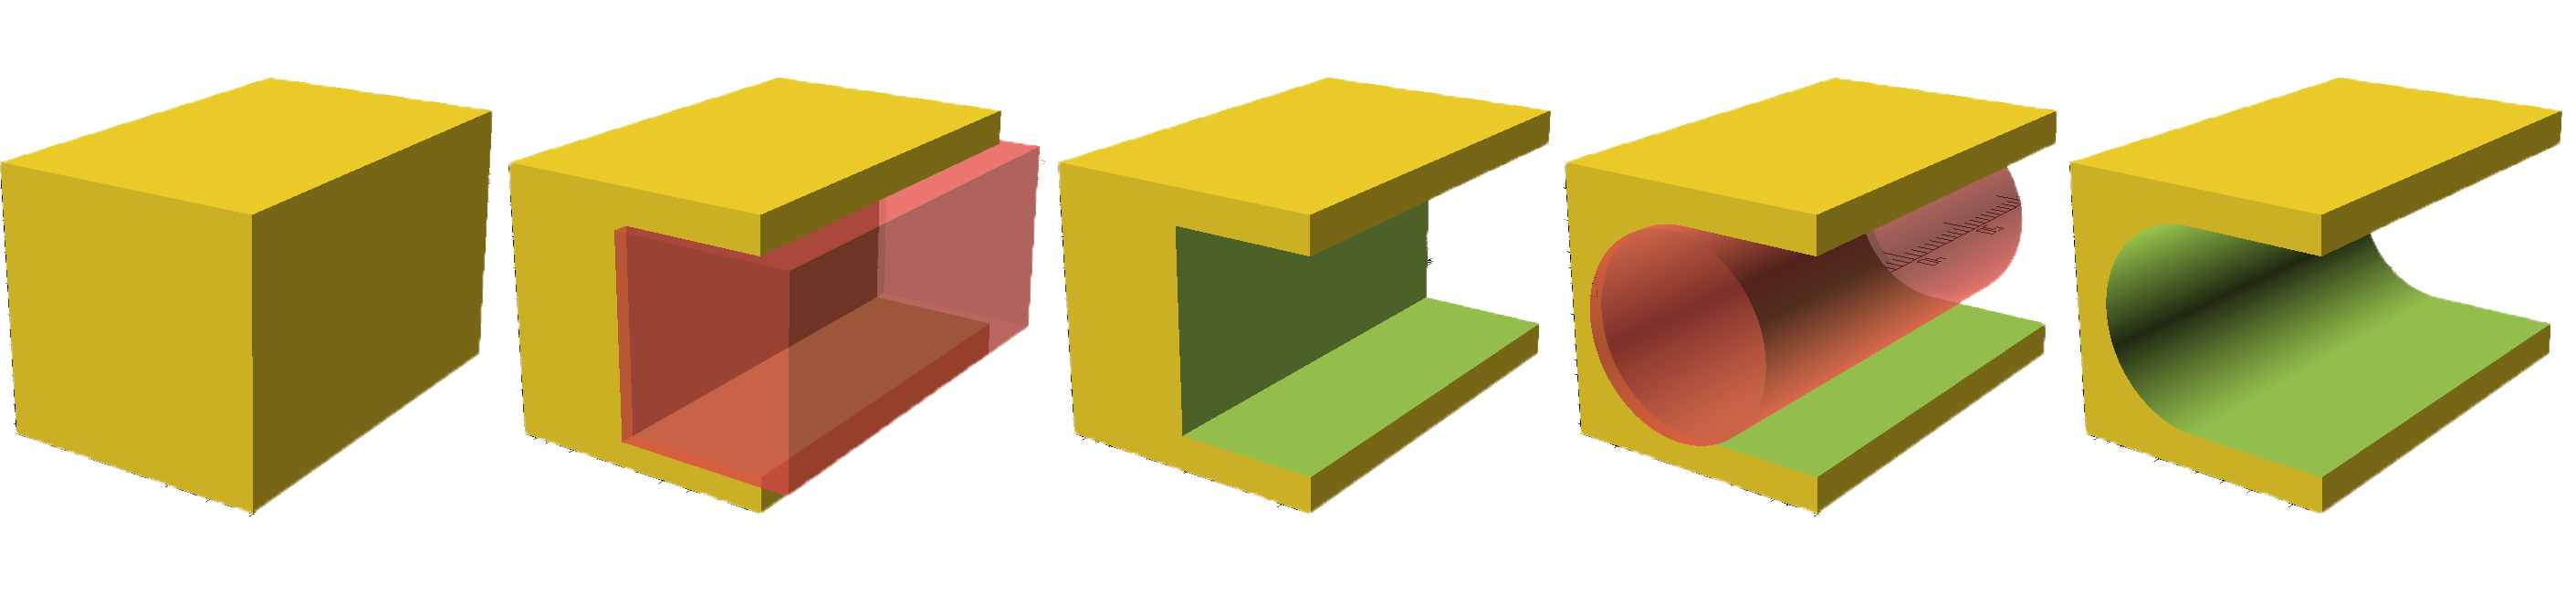
\includegraphics[width=\linewidth]{img/modelos/SoporteFeed/collageFeed.png}
    \caption{Construcción paso a paso del soporte del feed.}
    \label{fig:construcFeed}
\end{figure}

Durante la construcción del hueco cilíndrico de esta pieza surge un problema al intentar usar las medidas de Mallahzadeh: en la figura \ref{fig:esquemaFeed} (a) se indica que el hueco cilíndrico tiene un diámetro de 13 mm, es decir, radio $3/2=6.5$ mm; por otro lado, en \ref{fig:esquemaFeed} (b) se deduce que ese mismo radio es $(6-g)$ mm, siendo $g$ el grosor del soporte. Obviamente, siendo $g$ un número positivo es imposible que $6.5 = (6-g)$, por lo que o bien I) el perfil no es el de un cilindro, II) no es tangente con las partes de arriba y abajo del soporte o III) hay un error de acotación. Para poder avanzar en el modelo se ha supuesto que se debe a esto último, y se ha elegido un radio de $6.5$ mm. Tras esto sólo queda añadir el hueco cilíndrico para el cable coaxial.
\begin{figure}[!h]
    \centering
    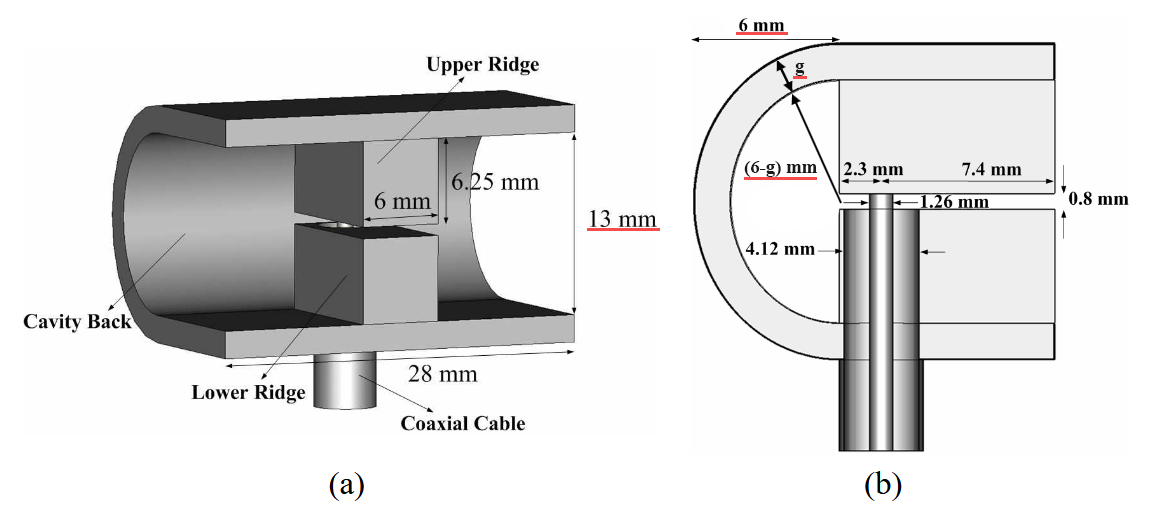
\includegraphics[width=0.9\linewidth]{img/modelos/SoporteFeed/feedEsquema.png}
    \caption{Esquema del feed de la antena \cite{tem_horn} con las anotaciones necesarias para ver el posible error de acotación subrayadas en rojo.}
    \label{fig:esquemaFeed}
\end{figure}

Una característica de OpenSCAD que ha acabado siendo muy útil a lo largo del proyecto es la posibilidad de parametrizar los tamaños y posiciones del modelo ya que, por ejemplo, se puede variar el grosor $g$ del soporte del feed manteniendo las distancias entre las demás piezas simplemente al cambiar el valor de una variable.\\

% ¿Contar los pasos de la impresión 3D o simplemente discutir los resultados y problemas?

\begin{wrapfigure}{r}{5.3cm}
    \vspace{-0.5cm}
    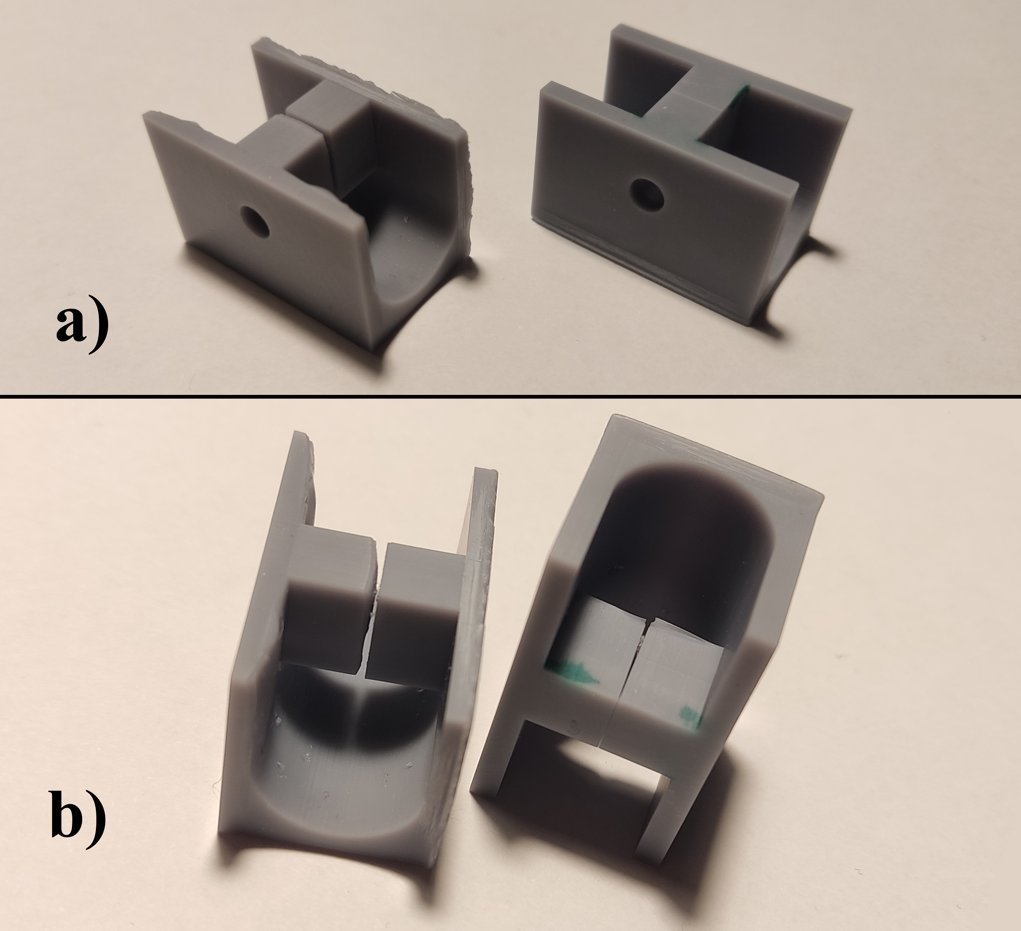
\includegraphics[width=\linewidth]{img/fotos/print1Cmprsd.png}
    \caption{Resultados de la primera prueba de impresión.}
    \label{fig:print1}
\end{wrapfigure}
Como resultado se obtuvieron las dos piezas de la figura \ref{fig:print1}. Como se puede apreciar en la subfigura (a), la pieza de la izquierda se imprimió apoyada sobre la cara opuesta al hueco para el cable, mientras que la pieza de la derecha se apoyó sobre su parte trasera. Esto ha dado lugar a diferentes errores de impresión (warping y delaminado) que se distinguen mejor en la subfigura (b).

Uno de los resultados más importantes de esta primera prueba de impresión es que dichos errores aparecen en planos paralelos al de impresión, por lo que en la medida de lo posible se evitarán las orientaciones paralelas a la dela pieza de la izquierda, ya que es importante para el funcionamiento de la antena que las dos caras del interior del feed permanezcan paralelas por esa zona.

%%%%%%%%%%%%%%%%%%%%%%%%%%%%%%%%%%%%%%%%%%%%%%%%%%%%%%%%%%%%%%%%%%%%%%%%%%%%%%%%
\subsection{Diseño de las placas - por segmentos}

La parte más externa de la construcción son las placas de la antena (o la antena en sí). En este caso se trata de dos placas que comienzan siendo paralelas entre sí y se curvan y ensanchan alejándose mutuamente, como se aprecia en la figura \ref{fig:esquemaPlacas}.
\begin{figure}[!h]
    \centering
    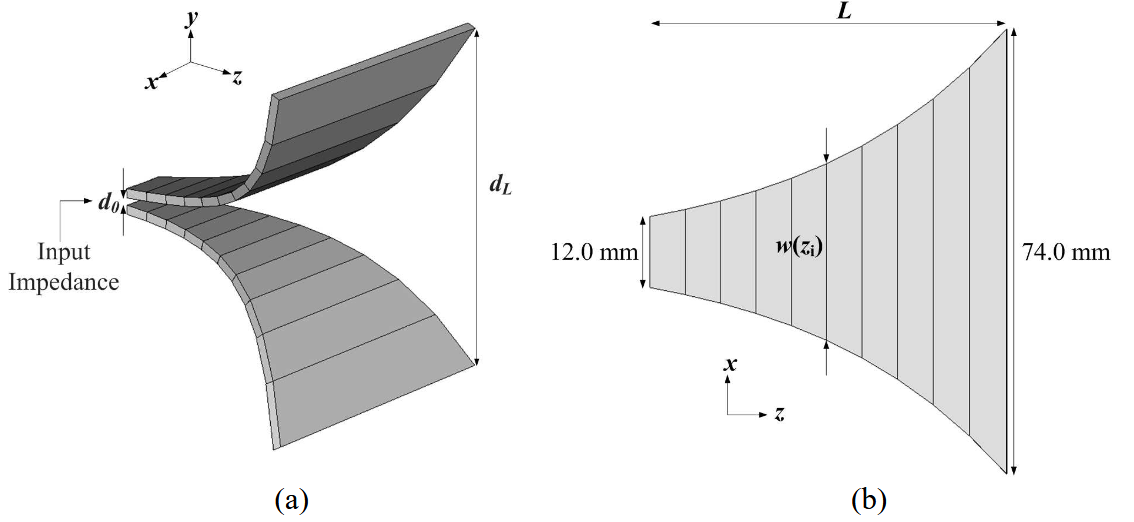
\includegraphics[width=\linewidth]{img/modelos/SoporteFeed/esquemaPlacas.png}
    \caption[Esquema de las placas de la antena \cite{tem_horn}.; (a) Vista 3D, (b) Proyección vertical.]
    {\tabular[t]{@{}l@{}}Esquema de las placas de la antena \cite{tem_horn}. \\ (a) Vista 3D; (b) Proyección vertical.\endtabular}
    \label{fig:esquemaPlacas}
\end{figure}

Para construirlas es necesario saber que la distancia entre placas de cada tramo viene dada por
\begin{equation}\label{eq:d(z)}
    d(z_i) = a\exp{(bz_i)}
\end{equation}
donde $z_i=iL/N$, y que la anchura $w(z_i)$ de cada tramo se obtiene de la impedancia característica
\begin{equation}\label{eq:w}
    \begin{cases}
        Z(z_i) = Z_0\exp (\alpha z_i)\\[5pt]
        Z(z_i) = \frac{d(z_i)}{w(z_i)}\eta
    \end{cases}
    \Rightarrow\hspace{0.1cm} w(z_i) = \frac{\eta a\exp (bz_i)}{Z_0\exp(\alpha z_i)} = \frac{\eta a}{Z_0}\exp [z_i(b-\alpha)]
\end{equation}
\noindent siendo las constantes
\begin{equation}
    a = d_0, \hspace{1.3cm} b=\frac{1}{L}\ln\left(\frac{d_L}{d_0}\right), \hspace{0.5cm}Z_0=50\text{ }\Omega, \hspace{0.5cm} \eta = 120\pi\text{ }\Omega, \hspace{0.5cm}\alpha = \frac{1}{L}\ln \frac{\eta}{Z_0}.
\end{equation}
\begin{wrapfigure}{r}{5.3cm}
    \vspace{-0.7cm}
    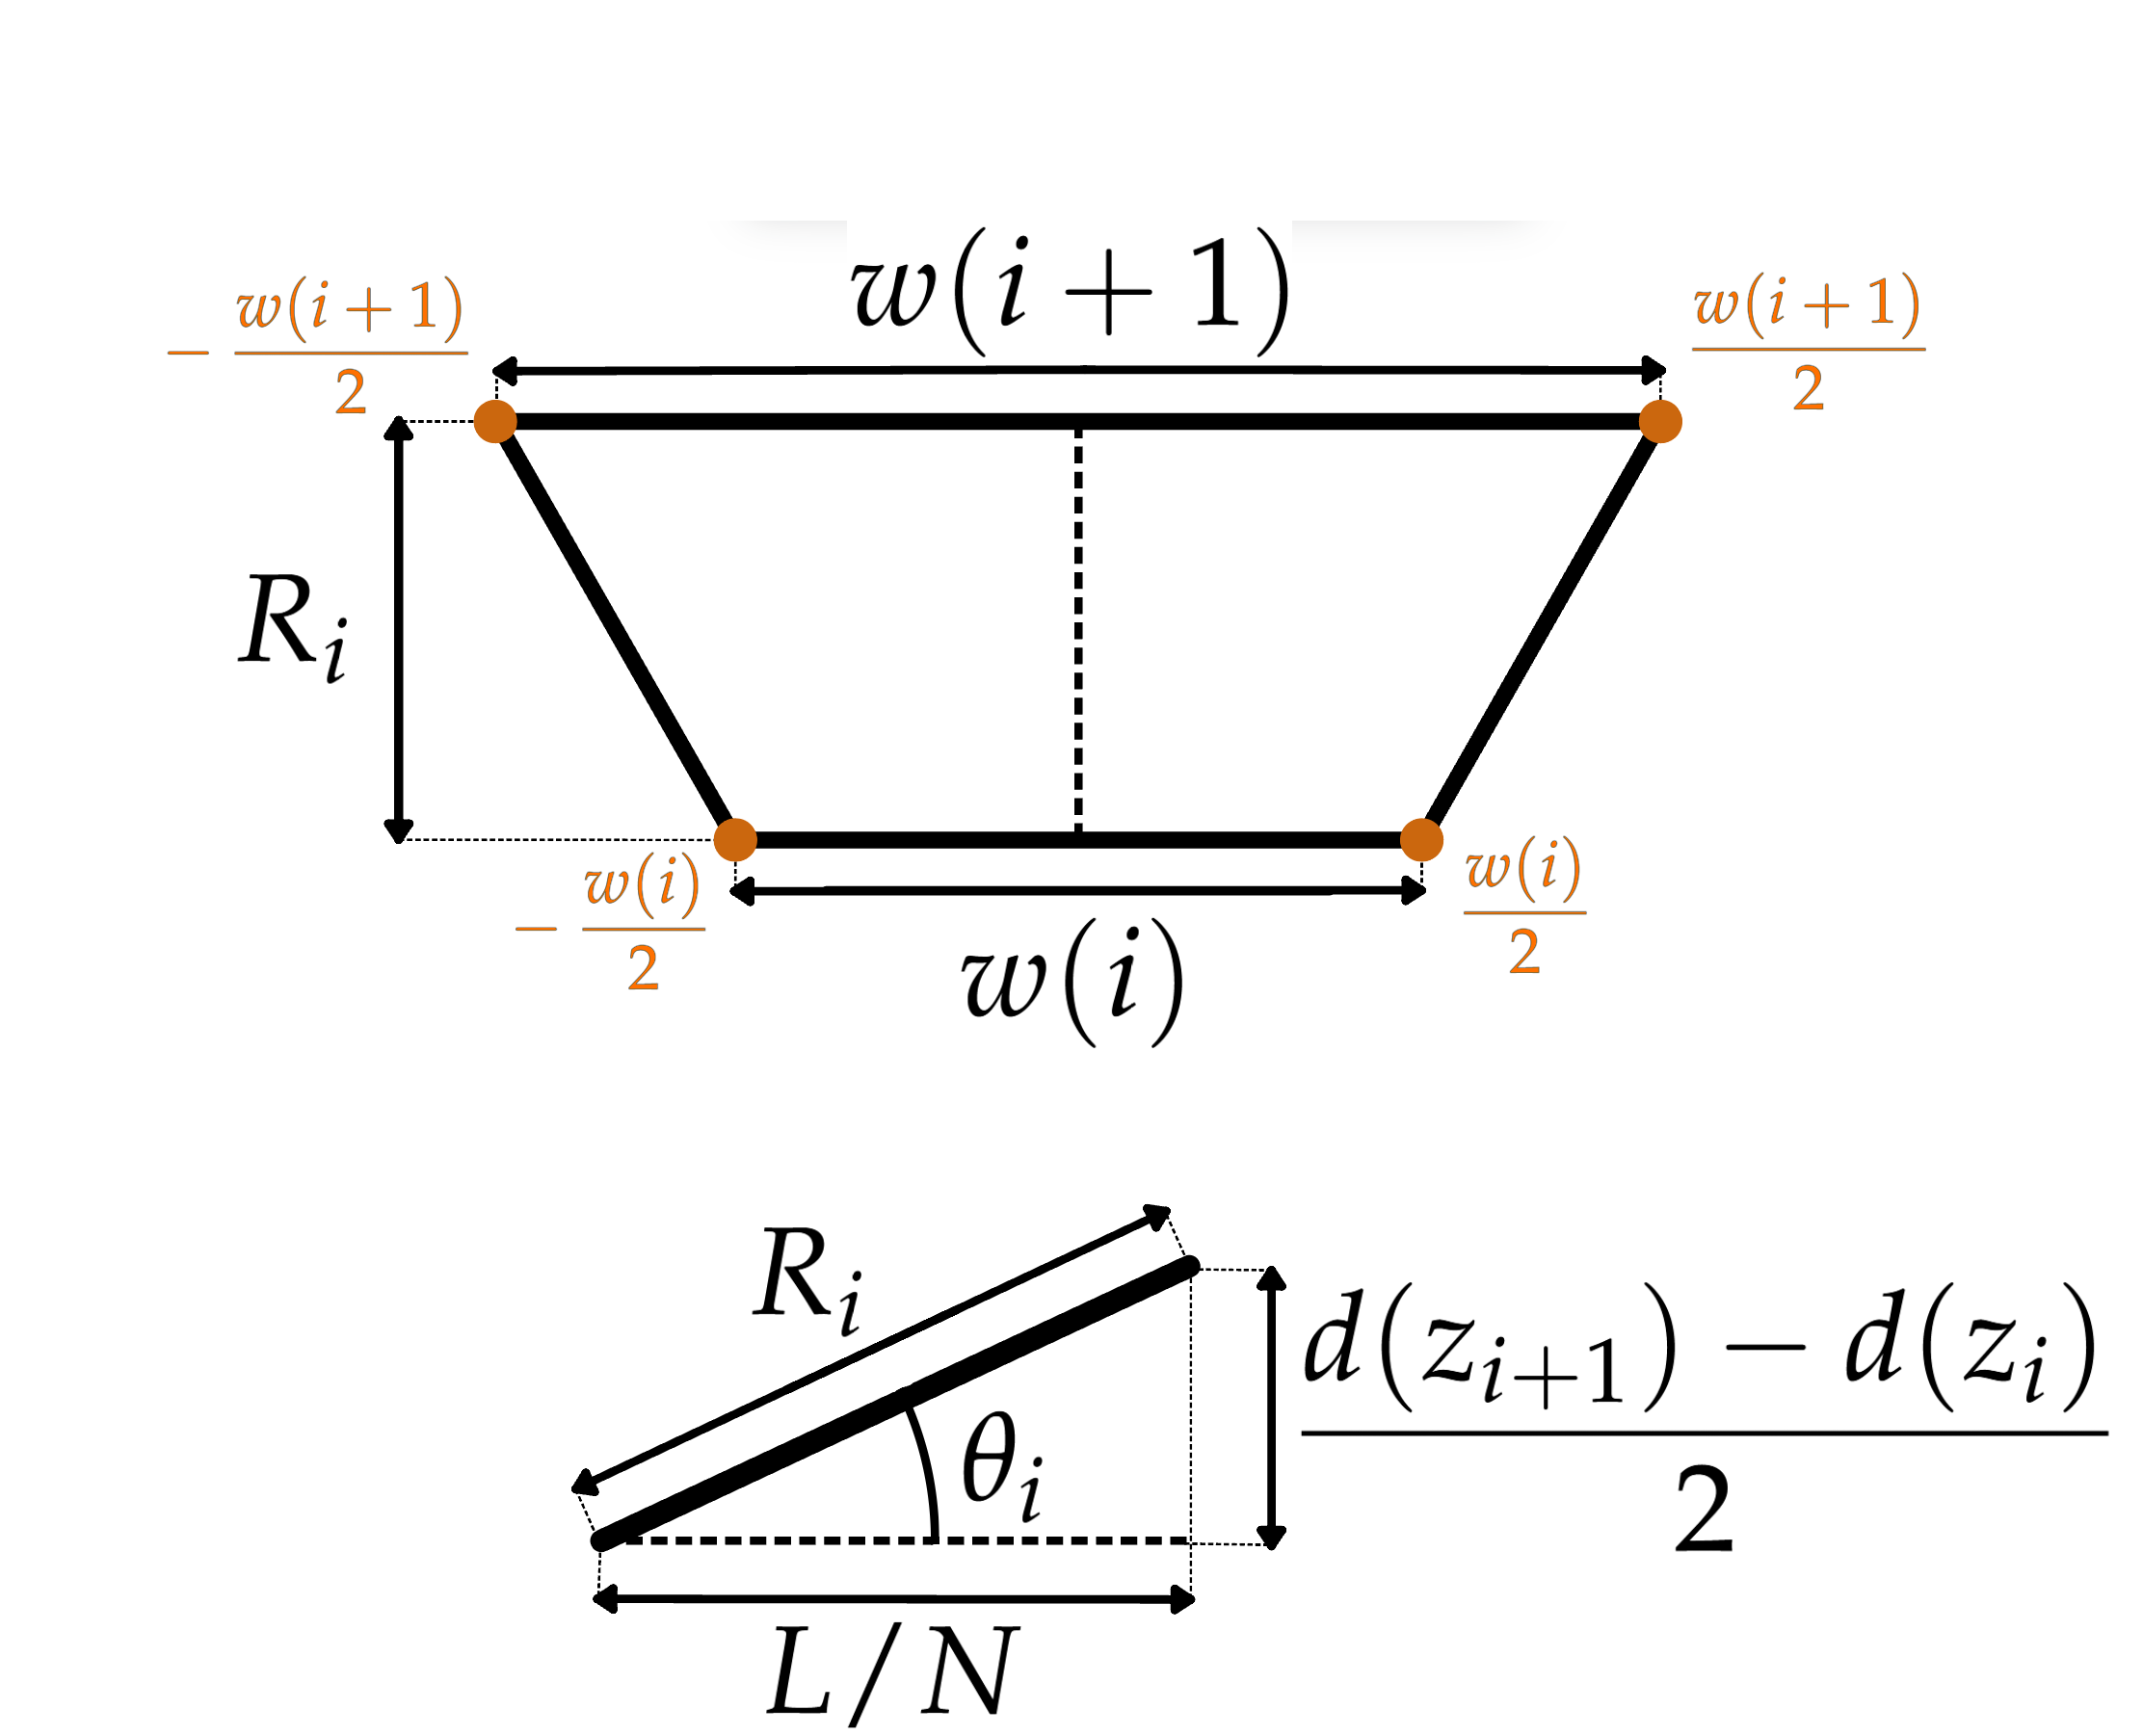
\includegraphics[width=\linewidth]{img/modelos/2025_02_20-Placas/schmPlacas.png}
    \caption{Magnitudes de cada segmento de las placas.}
    \label{fig:schmPlacas}
\end{wrapfigure}
El primer modelo para las placas de la antena se basa en la creación de los segmentos uno a uno. En la figura \ref{fig:schmPlacas} se indican los parámetros que se usarán para ello: $R_i$ es la altura del segmento $i$ y $\theta_i$ es el ángulo con el que se inclina.\\

Para construir cada uno de ellos se define un trapecio mediante sus cuatro vértices (color naranja en la figura \ref{fig:schmPlacas})

    \texttt{[[0,-w(i)/2],\hspace{1.55cm}[0,w(i)/2],}
    
    \texttt{[R(i+1),-w(i+1)/2],\hspace{0.2cm}[R(i+1),w(i+1)/2]]}
    
\noindent y luego se le hace una extrusión con el grosor deseado usando la función \texttt{extrude()}.\\

Una vez se han construido todas las placas de esta forma, se deben colocar con la orientación y posición correcta aplicando \texttt{rotate()} y \texttt{translate()}.\\

\begin{wrapfigure}{r}{5.3cm}
    \vspace{-0.4cm}
    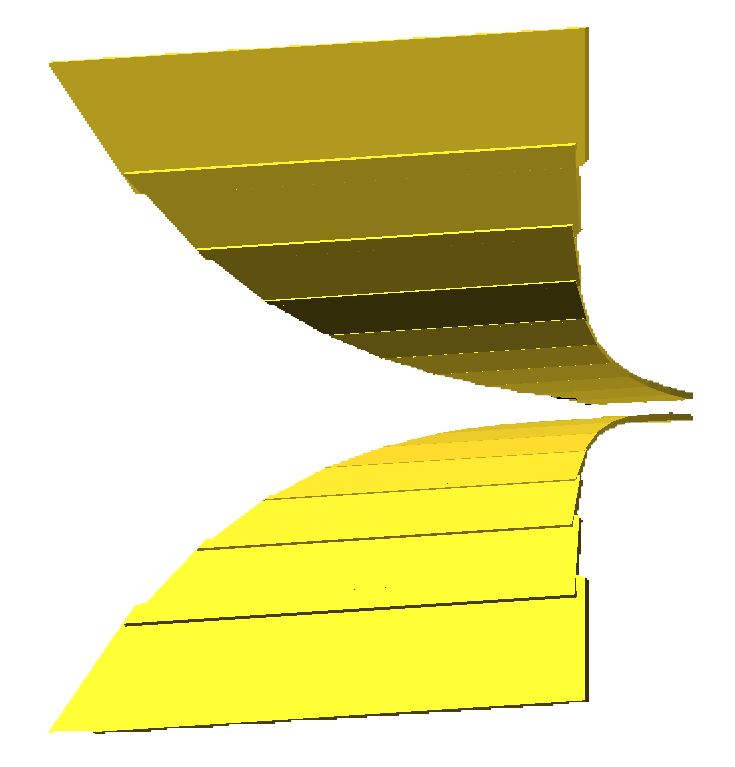
\includegraphics[width=\linewidth]{img/modelos/2025_02_20-Placas/picosPlacas.png}
    \caption{Resultado del método de construcción segmento a segmento.}
    \label{fig:segmentos}
\end{wrapfigure}
Con este método se pueden construir las placas mediante bucles tal que mediante un parámetro se elige el número de placas deseado y el resto de parámetros se ajustan automáticamente para que siempre se verifiquen las ecuaciones de arriba. 

No obstante, el problema aparece a la hora de colocar las placas: el lenguaje usado en OpenSCAD es un \textit{lenguaje funcional}, por lo que las variables no se pueden alterar dentro de bucles \texttt{for}. Como consecuencia, no es posible realizar la colocación de los segmentos mediante bucles, por lo que es necesario hacerlo uno a uno y se pierde el carácter paramétrico. Por otro lado, como se aprecia en la figura \ref{fig:segmentos}, la colocación manual de los segmentos es muy susceptible a fallos, un gran inconveniente cuando se tiene en cuenta que para el correcto funcionamiento de esta pieza es fundamental que no aparezcan bordes ni picos. 

Uno de los incentivos para realizar este proyecto es que, a diferencia del de Mallahzadeh, con nuestro método de construcción no hay ninguna complicación en crear placas con una gran cantidad de segmentos. El hecho de que haya que colocarlas una a una hace, de nuevo, que este diseño no sea el más adecuado.

%%%%%%%%%%%%%%%%%%%%%%%%%%%%%%%%%%%%%%%%%%%%%%%%%%%%%%%%%%%%%%%%%%%%%%%%%%%%%%%%
\subsection{Diseño de las placas - curvas}

Dado que el modelo anterior de las placas presenta serios inconvenientes, se crea uno nuevo basado también en la función \texttt{extrude()} pero con un procedimiento diferente que a continuación se explica paso a paso. Cada uno de estos pasos corresponde a una imagen de la figura \ref{fig:placasCurvas}:
\begin{figure}[!h]
    \centering
    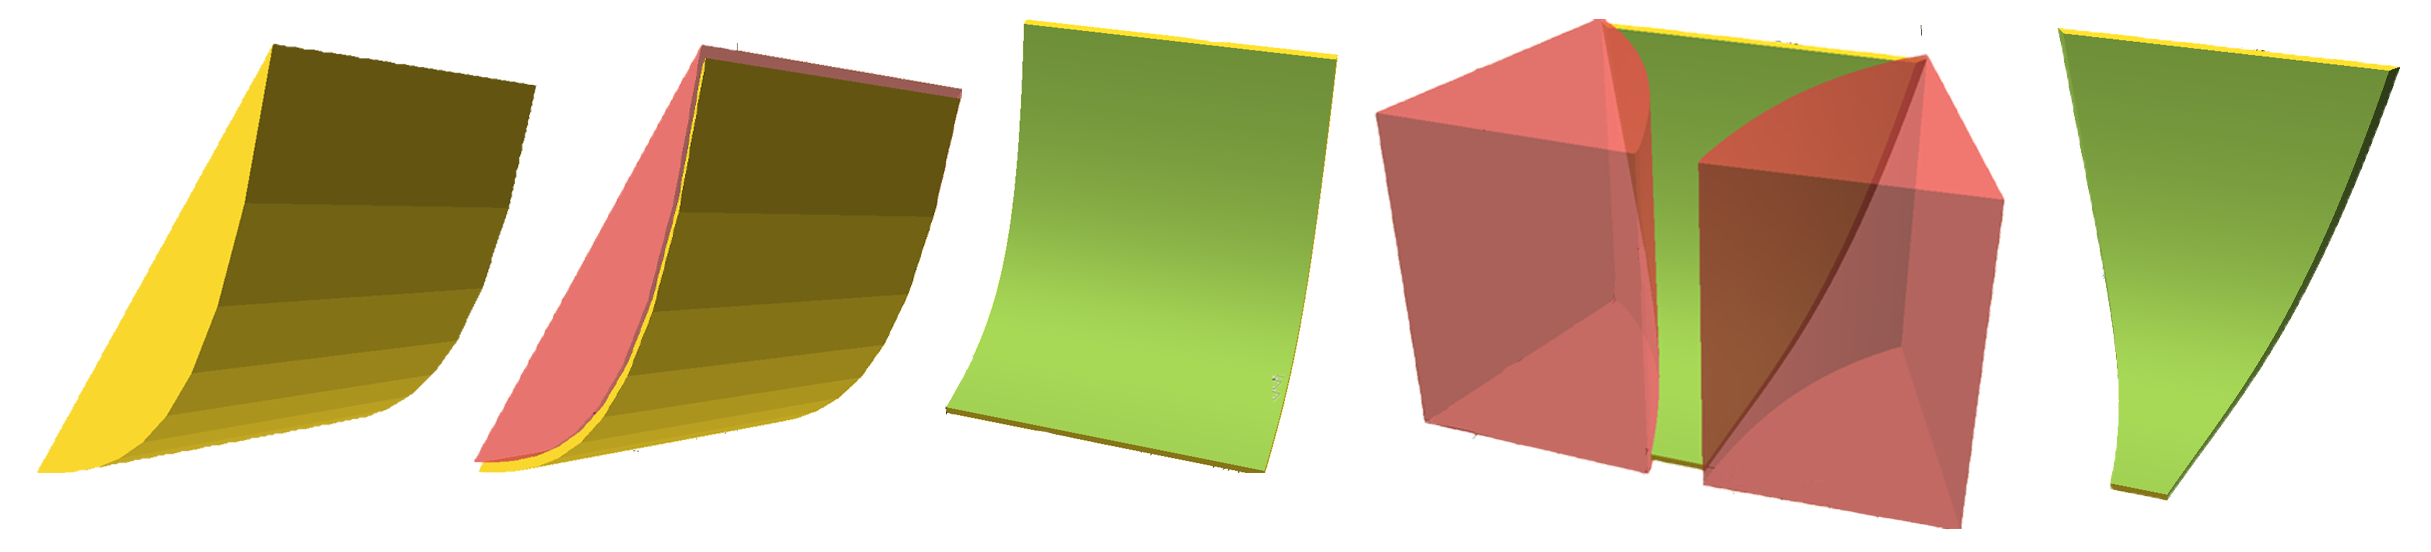
\includegraphics[width=\linewidth]{img/modelos/2025_02_21-ExtrudeFunctYSuavizado/placasCurvas.png}
    \caption{Creación de una placa paso a paso.}
    \label{fig:placasCurvas}
\end{figure}
\begin{itemize}
    \item[1.] Se crea un array con las posiciones de los puntos necesarios para crear el perfil lateral, con posiciones horizontales $z_i$ y verticales $d(z_i)$ (eq. \ref{eq:d(z)})
    \begin{minted}{python}
      // Generación de puntos - perfil vista lateral
      verticesF = [
          for (x = [0 : L/N : L])
              [x, a*pow(2.71828,b*x)/2],
          [0,L] // Para que la union con el feed sea buena
      ];
    \end{minted}
    y finalmente se extruyen los puntos del array \texttt{verticesF} para que la anchura total de la figura sea $w_{max}$.
    \begin{minted}{python}
        linear_extrude(height=wMax)
        polygon(points=verticesF);
    \end{minted}

    \item[2 y 3.] A la figura creada en el paso anterior se le resta una copia de sí misma ligeramente desplazada para dar como resultado una placa fina. Ajustando este desplazamiento se le da el grosor deseado a la placa.

    \item[4 y 5.] Finalmente se crean moldes con el perfil cenital que se restarán a la placa. Para ello, conociendo la expresión de la anchura de cada segmento (eq. \ref{eq:w}), se crean moldes a partir de una extrusión de la función $w(z)/2=\eta a e^{(b-\alpha)z}/2Z_0$ y se extruyen
    \begin{minted}{python}
      // Generación de puntos - perfil vista cenital
      verticesL = [
          for (x = [0 : L/N : L])
              [x, eta*a*pow(2.71828,(b-alpha)*x)/(2*Z0)],
          [0,L]
      ];
      (...)
      linear_extrude(height=wMax+2)
      polygon(points=verticesL);      
    \end{minted}
    Por último, solo queda restarlos a la placa colocándolos de manera adecuada.\\
\end{itemize}

\begin{wrapfigure}{r}{4.3cm}
    \vspace{-0.9cm}
    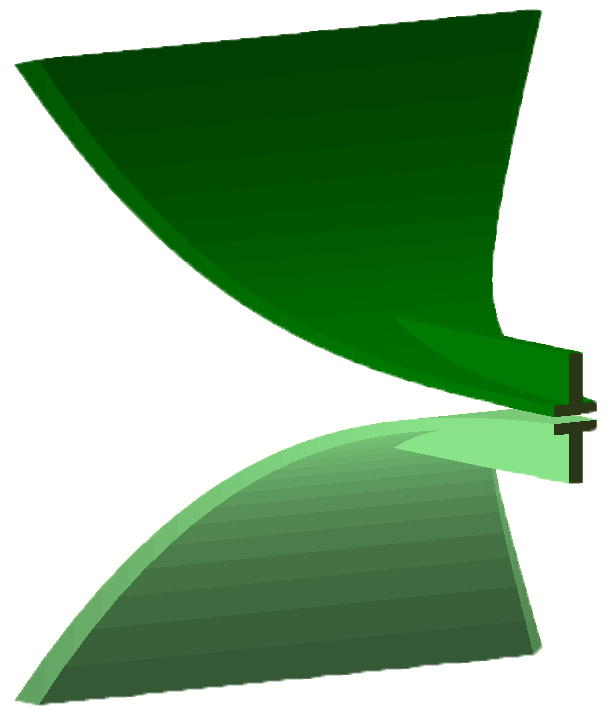
\includegraphics[width=\linewidth]{img/modelos/2025_02_21-ExtrudeFunctYSuavizado/cresta.png}
    \caption{Placas del segundo modelo.}\label{fig:cresta}
\end{wrapfigure}
En OpenSCAD, todo esto se hace dentro de un módulo para que el resultado final se pueda manejar de manera cómoda (trasladar, rotar, alterar parámetros, ...) sin tener que escribir todo el código cada vez.

Por otro lado, para que la placa sea más robusta y se fije mejor al soporte, se añade la cresta que se ve en la figura \ref{fig:cresta}.\\

Este modelo de placas soluciona los problemas que presentaba el anterior ya que no hay que colocar los segmentos manualmente tras su construcción, el diseño es completamente paramétrico y el código es mucho más fácil de interpretar si posteriormente tiene que modificarse.


%%%%%%%%%%%%%%%%%%%%%%%%%%%%%%%%%%%%%%%%%%%%%%%%%%%%%%%%%%%%%%%%%%%%%%%%%%%%%%%%
\subsection{Modelo II: Módulos}

La siguiente cuestión a resolver es cómo metalizar correctamente las placas y el hueco del conector. El principal inconveniente que aparece al construirlo de la forma actual es que durante el metalizado será muy complicado aplicar el spray correctamente por la parte interior del hueco y entre las placas. Para resolver esto, se separa la antena en tres módulos que se metalizan por separado y luego se ensamblan encajándolos en orden, como se indica en la figura \ref{fig:modulos}.
\begin{figure}[!h]
    \centering
    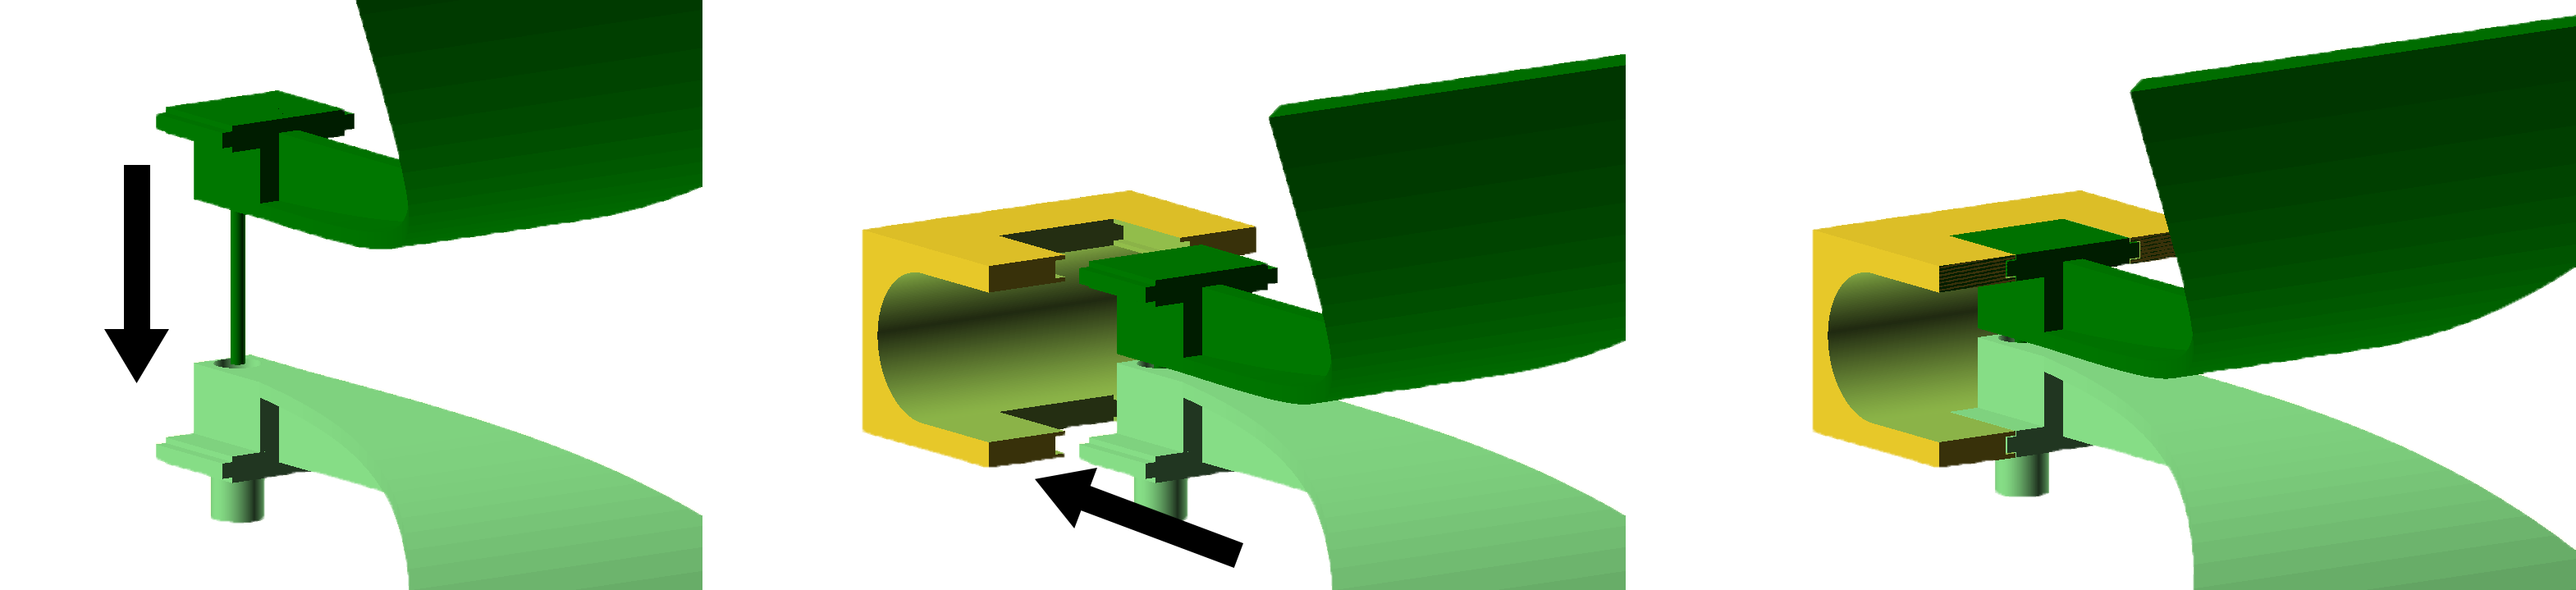
\includegraphics[width=\linewidth]{img/modelos/2025_02_25-Ranuras/cunias.png}
    \caption{Esquema del montaje de los módulos de la antena.}
    \label{fig:modulos}
\end{figure}

Para construirlo en OpenSCAD se crea una extrusión de un polígono para dar lugar a la pieza que aparece marcada en rojo en la figura \ref{fig:molde}. Esta pieza se resta al soporte del feed y luego se escala para hacerse ligeramente más pequeña y se añade a ambas placas de la antena para que pueda encajar.
\begin{figure}[!h]
    \centering
    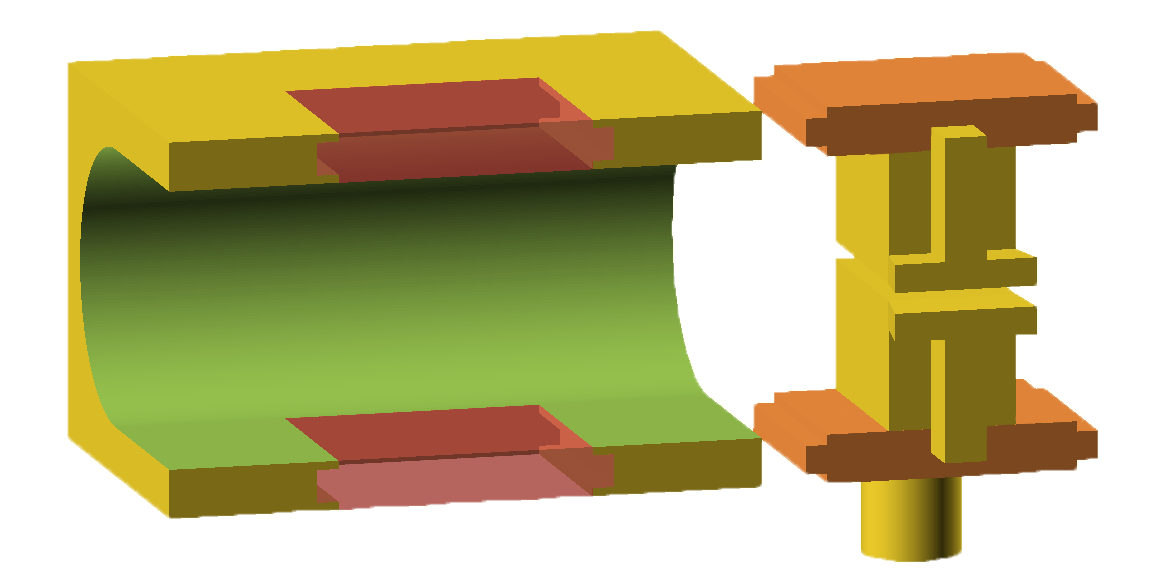
\includegraphics[width=0.7\linewidth]{img/modelos/2025_02_25-Ranuras/molde.png}
    \caption{Componentes de la ranura marcados en rojo y en naranja.}
    \label{fig:molde}
\end{figure}

Como resultado de la impresión se obtuvieron las piezas de la figura \ref{fig:modulosPrint}. Como el objetivo de esta prueba de impresión era comprobar si las piezas encajan y se sostienen correctamente, no se imprimieron las placas de la antena. En el modelo 3D el hueco que queda al encajar las piezas se ha elegido de $0.1$ mm, y el resultado es un agarre firme y sin holgura.

Este modelo da lugar a un diseño modular que resultará muy conveniente en la fase de metalización y permitirá sustituir partes de la antena en caso de que no funcionen sin necesidad de rehacerla desde cero.
\begin{figure}[!h]
    \centering
    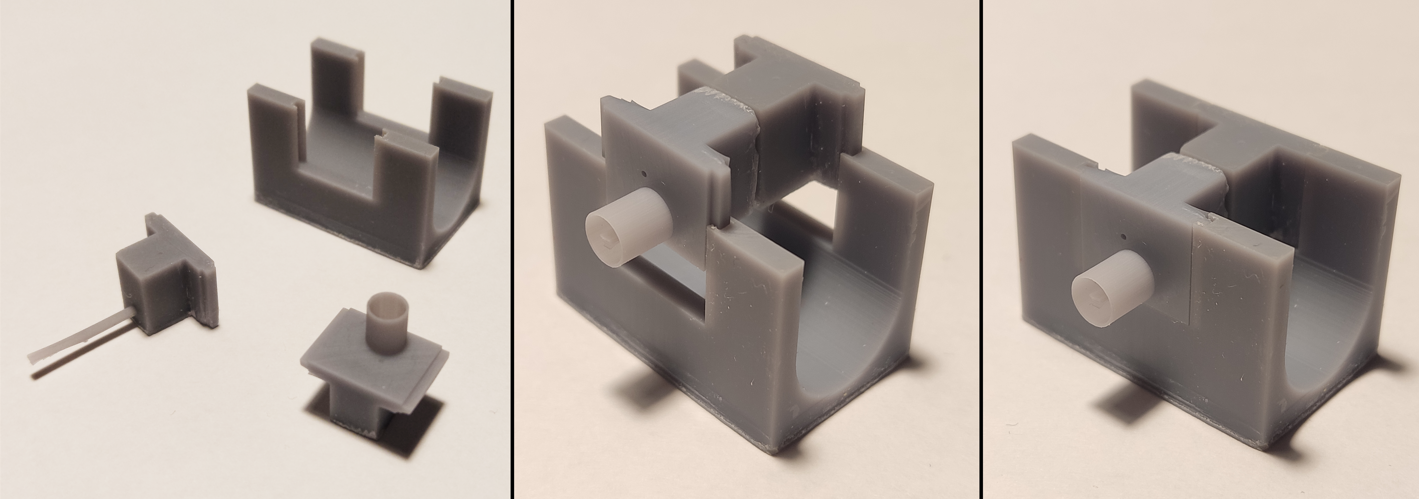
\includegraphics[width=\linewidth]{img/modelos/2025_02_25-Ranuras/modulosPrint.png}
    \caption{Resultados de la segunda prueba de impresión.}
    \label{fig:modulosPrint}
\end{figure}

%%%%%%%%%%%%%%%%%%%%%%%%%%%%%%%%%%%%%%%%%%%%%%%%%%%%%%%%%%%%%%%%%%%%%%%%%%%%%%%%
\subsection{Modelo III: Conector}

%%%%%%%%%%%%%%%%%%%%%%%%%%%%%%%%%%%%%%%%%%%%%%%%%%%%%%%%%%%%%%%%%%%%%%%%%%%%%%%%
%%%%%%%%%%%%%%%%%%%%%%%%%%%%%%%%%%%%%%%%%%%%%%%%%%%%%%%%%%%%%%%%%%%%%%%%%%%%%%%%
\section{Simulación}



%%%%%%%%%%%%%%%%%%%%%%%%%%%%%%%%%%%%%%%%%%%%%%%%%%%%%%%%%%%%%%%%%%%%%%%%%%%%%%%%
%%%%%%%%%%%%%%%%%%%%%%%%%%%%%%%%%%%%%%%%%%%%%%%%%%%%%%%%%%%%%%%%%%%%%%%%%%%%%%%%
\section{Conclusiones}

Esta sección no debería faltar en todo TFG. Después van las referencias que pueden añadirse en la misma página o en una nueva, como se ha hecho aquí. Hay ejemplos de cómo deben citarse artículos, ...

% Referencias %%%%%%%%%%%%%%%%%%%%%%%%%%%%%%%%%%%%%%%%%%%%%%%%%%%%%%%%%%%%%%%%%
%\newpage

\addcontentsline{toc}{section}{Referencias} % Elige según idioma
%\addcontentsline{toc}{section}{References} % Elige según idioma

\begin{thebibliography}{100}

\bibitem{tem_horn}
A.~R.~Mallahzadeh and F.~Karshenas, \\
{\em Modified TEM Horn Antenna for Broadband Applications}, \\
Progress In Electromagnetics Research, PIER 90, 105--119, 2009.

 
\end{thebibliography}

\end{document}

